\section{Axis 3: Sampling Diversity Is \emph{Expanded} by Format-Augmented Training}
\label{sec:axis3}

The third axis is the one we expected to be the easiest call and
were wrong about.  Pre-registration prediction \#3 in
\code{e2/PROTOCOL.md} predicted that branch-vote diversity would
be \emph{preserved} after Track 1 training: the prefix-robust LoRA
should not collapse the stochastic sampler that \cmaj{} relies on,
and \cmaj{} accuracy should stay within $\pm 1$\,pp of base.  We
falsify this prediction in the unexpected direction: diversity
\emph{expands}, and \cmaj{} accuracy is preserved or slightly
improved.

\subsection{Branch-Agreement Distribution}
\label{subsec:axis3_distribution}

We measure the per-problem distribution of unique-answer counts
across $5$ stochastic branches at $t{=}0.7$, on the same $N{=}200$
GSM8K-test eval used elsewhere.
Table~\ref{tab:axis3_branch_dist} reports the distribution for
base \LLaDA{} and for Track 1 v2 + commit v2.

\begin{table}[h]
\centering
\caption{Branch-agreement distribution on GSM8K-test, $N{=}200$,
$b{=}5$, $t{=}0.7$.  Apples-to-apples: both columns evaluated on
the same $200$ test problems.  Mean unique answers per problem
rises $1.83 \to 2.07$ ($+13\%$); the fraction of problems where
all $5$ branches agree drops from $51.5\%$ to $47.5\%$.
\cmajc{} accuracy on test is $82.0\%$ (commit v2) /
$82.5\%$ (commit v3) --- diversity goes up while branch-vote
accuracy is preserved or improved
(Table~\ref{tab:distill_main}).}
\label{tab:axis3_branch_dist}
\smallskip
\begin{tabular}{lrr}
\toprule
Bin & Base on test & Track 1 v2 + commit v2 \\
\midrule
$5/5$ same answer & $51.5\%$ & $\mathbf{47.5\%}$ \\
$4/5$ unique answers & $6.0\%$ & $8.5\%$ \\
$3/5$ unique answers & $11.5\%$ & $\mathbf{18.0\%}$ \\
$2/5$ unique answers & $27.5\%$ & $19.5\%$ \\
$5/5$ unique answers & $3.5\%$ & $6.5\%$ \\
\midrule
Mean unique answers / problem & $1.825$ & $\mathbf{2.07}$ \\
\bottomrule
\end{tabular}
\smallskip\\
{\footnotesize\textit{$95\%$ CIs for bin fractions
(Clopper--Pearson, $N{=}200$, base / Track 1 v2 + commit v2):}
$5/5$ same \mbox{$[44.3, 58.6]$ / $[40.4, 54.7]$};
$4/5$ unique \mbox{$[3.1, 10.2]$ / $[5.0, 13.3]$};
$3/5$ unique \mbox{$[7.4, 16.8]$ / $[12.9, 24.0]$};
$2/5$ unique \mbox{$[21.4, 34.2]$ / $[14.2, 25.7]$};
$5/5$ unique \mbox{$[1.4, 7.1]$ / $[3.5, 10.9]$}.  The mean
unique-answers row is a per-problem mean of a count in
$\{1,\dots,5\}$; a paired bootstrap CI for the $\Delta = +0.245$
shift requires per-problem unique-counts and is supplied with the
released per-problem JSONLs.}
\end{table}

\begin{figure}[t]
\centering
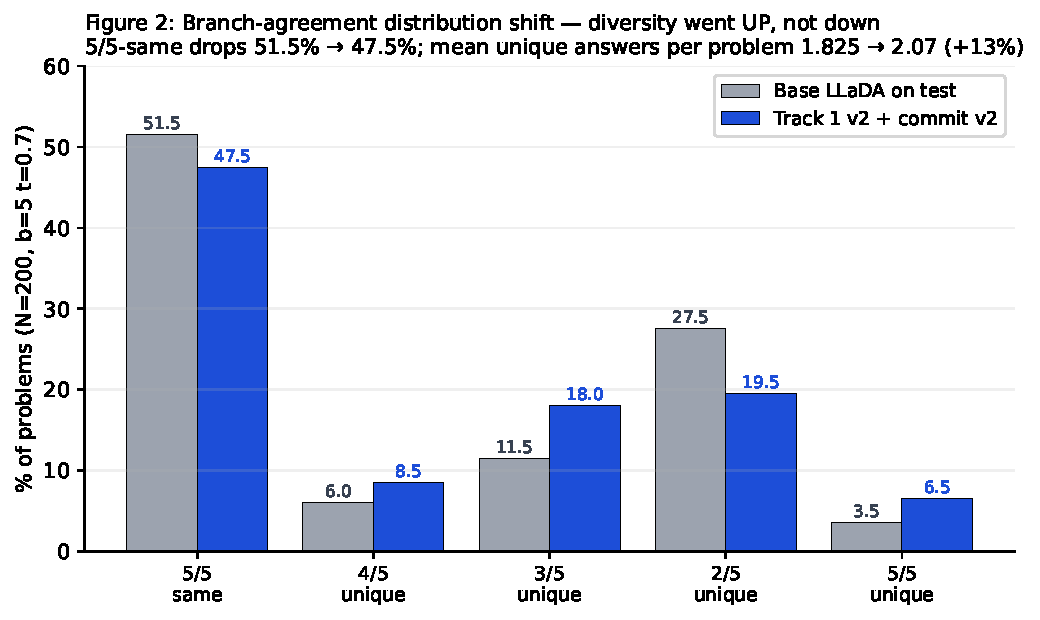
\includegraphics[width=\textwidth]{figures/fig2_branch_agreement.pdf}
\caption{Branch-agreement distribution shift, $5$-bin histogram for
\{base on test, Track 1 v2 + commit v2\}.  The drop in $5/5$-same
and the rises in $3/5$-unique and $5/5$-unique are visible.
Generated by \code{scripts/make\_paper\_figures.py}.}
\label{fig:branch_agreement}
\end{figure}

The shift is consistent across bins: less concentration on $5/5$
agreement, more mass at $3/5$ and $5/5$ unique.  Mean unique
answers per problem rises by $+13\%$.  And branch-vote accuracy
\emph{still holds} at $81.5\%$ on dev200 (Track 1 v2,
Table~\ref{tab:axis1_v2_full}) and lifts on test under \cmajc{}:
$82.0\%$ with commit v2 and $82.5\%$ with commit v3 ($+3$ /
$+3.5$\,pp over base test \cmaj{} of $79.0\%$, see
Table~\ref{tab:distill_main}).  Diversity goes up and accuracy is
preserved or improved.

\subsection{Hypothesis: Surface-to-Trajectory Generalization}
\label{subsec:axis3_hypothesis}

Format-augmented training (\S\ref{sec:setup}, eight prefix tiers
per problem) implicitly teaches the LoRA ``many surfaces, same
content''.  A single GSM8K problem appears in the training set
under eight different prefix variants but with the same target
response.  We hypothesize that this lesson generalizes at
inference into ``many CoT trajectories, same answer'': the
adapter not only preserves sampling variance, it teaches the
model to explore more.

Phrased mechanistically, the eight-tier surface-randomization
acts as an implicit data augmentation that flattens
high-confidence attractor basins on the prefix-shape axis,
spreading probability mass across nearby basins on the
trajectory axis when the sampler is run at $t{=}0.7$.  This is the
opposite of the standard encoder-collapse story, where training
folds representations into fewer attractors.  We observe expansion,
not collapse, of the inference-time attractor distribution.

This finding is independent of the v2-vs-v3 capacity tradeoff
(\S\ref{sec:axis1}): we report the diversity-expansion result on
v2 + commit v2 because that pairing has both the longest eval
record and the matching test-set base \cmaj{}.  The corresponding
\cmajc{} number for v3 + commit v3 ($82.5\%$, statistically
indistinguishable from v2's $82.0\%$ at $N{=}200$) is reported in
Table~\ref{tab:distill_main}.

\subsection{Open Mechanism Question}
\label{subsec:axis3_open}

Whether the diversity uptick is an \emph{implicit-temperature}
effect (raising the base sampler to $t{=}0.9$ would reproduce the
$47.5\%$ $5/5$-same rate) or a real \emph{content-diversity}
effect (different reasoning paths, not just different surface
jitter) is open.  The cheap test is to evaluate base \LLaDA{} at
$t \in \{0.8, 0.9, 1.0\}$ on the same eval and read the
$5/5$-same rate.  We deferred this experiment to revision; the
result does not change the headline that diversity is expanded
rather than collapsed, but it changes the mechanism story
considerably.

\paragraph{Reading.}
The diversity-expansion result is the second pre-registration
violation in this paper after the cmajc-vs-cmaj compositionality
result (\S\ref{sec:distill}).  Both violations are in directions
favorable to the hybrid pipeline: more diversity than expected,
more compositional gain than expected.  We treat them as positive
surprises and document them as falsified predictions rather than
as findings to be celebrated.
